\section{ProgC}

    \subsection{Wichtige Kurzbefehle}
		\begin{tabular}{ll}
			\verb|cd "Path"| & Pfad anwählen \\
			\verb|cd ..| & um eine Ebene nach oben (zurück) \\
			\verb|mkdir "Ordnername"| & Ordner erstellen \\
			\verb|rmkdir "Ordnername"| & Ordner löschen \\
			\verb|rm -rf *| & Alles innerhalb vom aktuellen Ordner löschen \\
			\verb|rm "Datei"| & Datei löschen \\
			\verb|mv "Name alt" "Name neu"| & Datei umbenennen \\
			\verb|cp "Datei alt" "Datei neu"| & Datei kopieren und benennen \\
			\verb|clang -Wall -o "Outputname" "Inputdatei"| & clang-Compiler mit Warnungen \\
			\verb|clang -Wall -o "Outputname" "Inputdatei" -lm| & -lm für Mathebibliothek \\
			\verb|ls| & Listet alle Files im akt. Verzeichnis auf \\
			\verb|ls -l| & Inkl. Informationen wie Grösse u.a. \\
			\verb|ls -a| & Inkl. versteckten Dateien \\
			\verb|ls -al| & Beide Varianten \\
		\end{tabular}

	\subsection{Zahlensysteme}
		\begin{tabular}{|l|l|l|l|l|l|l|l|}
			\hline
			$2^0$ = 1 & $2^1$ = 2 & $2^2$ = 4 & $2^3$ = 8 & $2^4$ = 16 & $2^5$ = 32 & $2^6$ = 64 & $2^7$ = 128 \\
			\hline
		\end{tabular}

		\begin{tabular}{|l|l|l|l|}
			\hline
			\textbf{Grösse} & \textbf{Abk.} & \textbf{Genauer Wert} & \textbf{Näherung} \\
			\hline
			Kilobyte & kB & $2^{10}$ = 1024 Bytes & $10^3$ Bytes \\
			\hline
			Megabyte & MB & $2^{20}$ = 1 048 576 Bytes & $10^6$ Bytes \\
			\hline
			Gigabyte & GB & $2^{30}$ = 1 073 741 824 Bytes & $10^9$ Bytes \\
			\hline
			Terabyte & TB & $2^{40}$ = 1 099 511 627 776 Bytes & $10^12$ Bytes \\ 
			\hline
		\end{tabular}

		\begin{tabular}{|l|llllll|}
			\hline
			Oktal & 3 Bits & $X_8$ & $X_O$ & $X_q$ & $X_oct$ & $0X$ \\
			\hline
			Hex & 4 Bits   & $X_16$ & $X_h$ & $XH$ & $X_hex$ & 0xX \\
			\hline
		\end{tabular}

		\paragraph{Hexadezimal}
			\begin{tabular}{llllllllllllllll}
				0 & 1 & 2 & 3 & 4 & 5 & 6 & 7 & 8 & 9 & 10 & 11 & 12 & 13 & 14 & 15 \\
				0 & 1 & 2 & 3 & 4 & 5 & 6 & 7 & 8 & 9 & A & B & C & D & E & F \\
			\end{tabular}
			
		\paragraph{ASCII (7-Bit)}
			
			Ordnet gängigen Schriftzeichen einen Zahlenwert zu, um diese in einem Digitalrechner präsentieren zu können.
			Die Tabelle ist wichtig, um für geg. Schriftzeichen den repräsentierten Zahlenwert zu ermitteln (und umgekehrt).

			Nachfolger: Unicode (8-, 16-, 32-Bit)
	
	\subsection{Datentypen}
		\subsubsection{Datentypen}
			\begin{tabular}{lll}
				\textbf{Ganzzahltypen} & & \\
				char      & Buchstaben, Zahlen & 8 Bit (1 Byte) \\
				short     & kleine, ganzz. Werte & abh. (min 16bit) \\
				int       & eff. Grösse des Prozessors & abh. (min 16bit) \\
				long      & grosse ganzz. Werte & abh. (min 32bit) \\
				long long & sehr grosse ganzz. Werte & abh. (min 64bit) \\
				\textbf{Gleitpunkttypen} & & \\
				float     & Gleitpunkt, single precision & abh. \\
				double    & Gleitpunkt, high precision, Standard & abh. \\
				long double & Gleitpunkt, higher precision & abh. \\
				& & \\
				\textbf{Platzhalter} & & \\
				char                   & \verb|%c| & l, ll $>$ Typ länger als ein \verb|int| \\
				Zeichenkette           & \verb|%s| & h, hh $>$ Typ kürzer als ein \verb|int| \\
				Signed Ganzzahl dez.   & \verb|%d| & \\
				Unsigned Ganzzahl dez. & \verb|%u| & \\
				Unsigned Ganzzahl okt. & \verb|%o| & \\
				Unsigned Ganzzahl hex. & \verb|%x| & \\
			\end{tabular}
			
			\textbf{Ganzzahlen} können überlaufen!

			\textbf{Gleitpunktzahlen} haben meist Rundungsfehler. Nie auf Gleichheit prüfen!

		\subsubsection{Typumwandlung}
			\verb|float f = 41.7;|\\
			Implizit: Eine Kommazahl ohne \verb|f| am Ende hat den Typ \verb|double|
			\\
			\\
			\verb|int x = (int) f;|\\
			Explizit: x hat den Wert 41, Nachkommastellen werden abgeschnitten

		\subsubsection{Namen}

		\subsubsection{Wertebereich}
			\begin{tabular}{lll}
				unsigned & 0...$(2^n-1)$               & n=8 : 0...255 \\
				signed   & $-2^{n-1}...+(2^{n-1}-1)$ & n=8 : -128...+127 \\
			\end{tabular}
		
	\subsection{Variablen}
		\begin{minipage}{1\linewidth}
			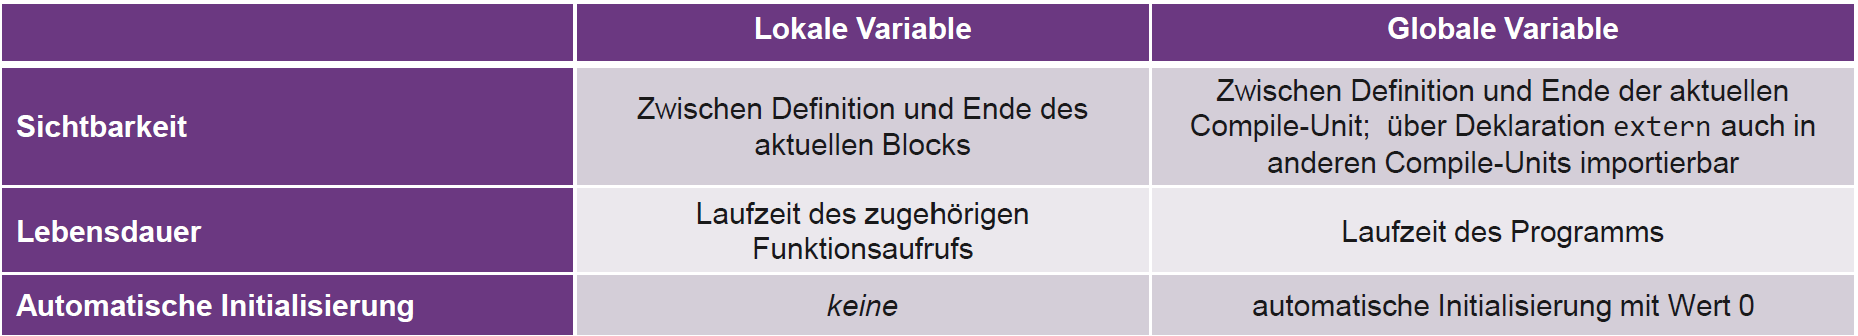
\includegraphics[width=1\linewidth]{Bilder/sichtbarkeit_variablen.png}
		\end{minipage}

	\subsection{Schleifen}
		\begin{itemize}
			\item \verb|for|-Schleife: Für Zählschleifen, bzw. wenn die Anzahl Durchläufe bekannt ist
			\item \verb|do...while|-Schleife: Keine Zählschleife, min. 1 Durchlauf
			\item \verb|while|-Schleife: In allen anderen Fällen	
		\end{itemize}

		\subsubsection{For-Schleife}
			\begin{minipage}{.45\linewidth}
				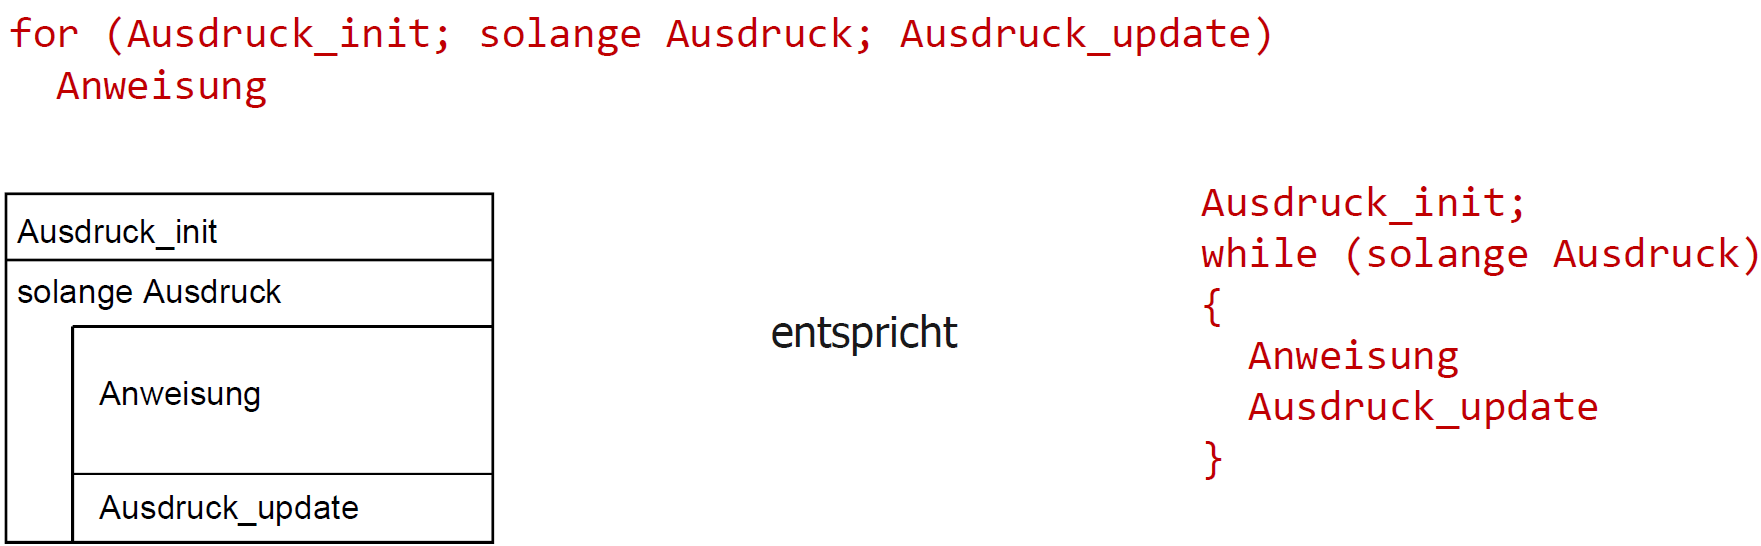
\includegraphics[width=0.95\linewidth]{Bilder/forschleife.png}
			\end{minipage}
			\hfill
			\begin{minipage}{.5\linewidth}
				For-Schleife
			\end{minipage}

		\subsubsection{Switch-Schleife}
			\begin{minipage}{.45\linewidth}
				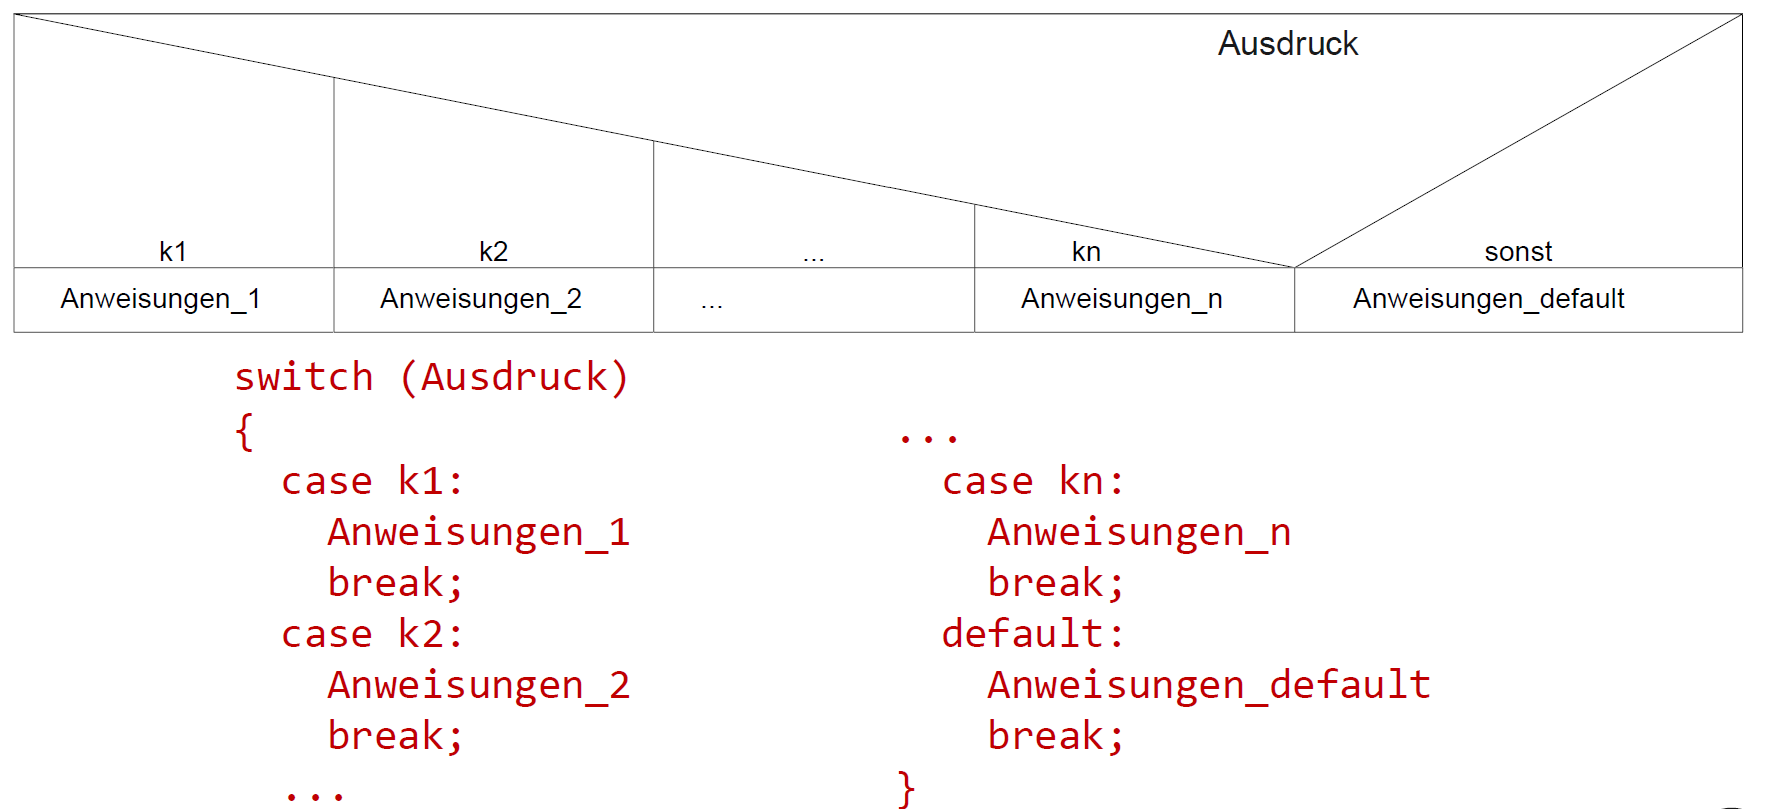
\includegraphics[width=0.95\linewidth]{Bilder/Switch.png}
			\end{minipage}
			\hfill
			\begin{minipage}{.5\linewidth}
				Switch-Schleife
			\end{minipage}

		\subsubsection{Do-While-Schleife}
			\begin{minipage}{.45\linewidth}
				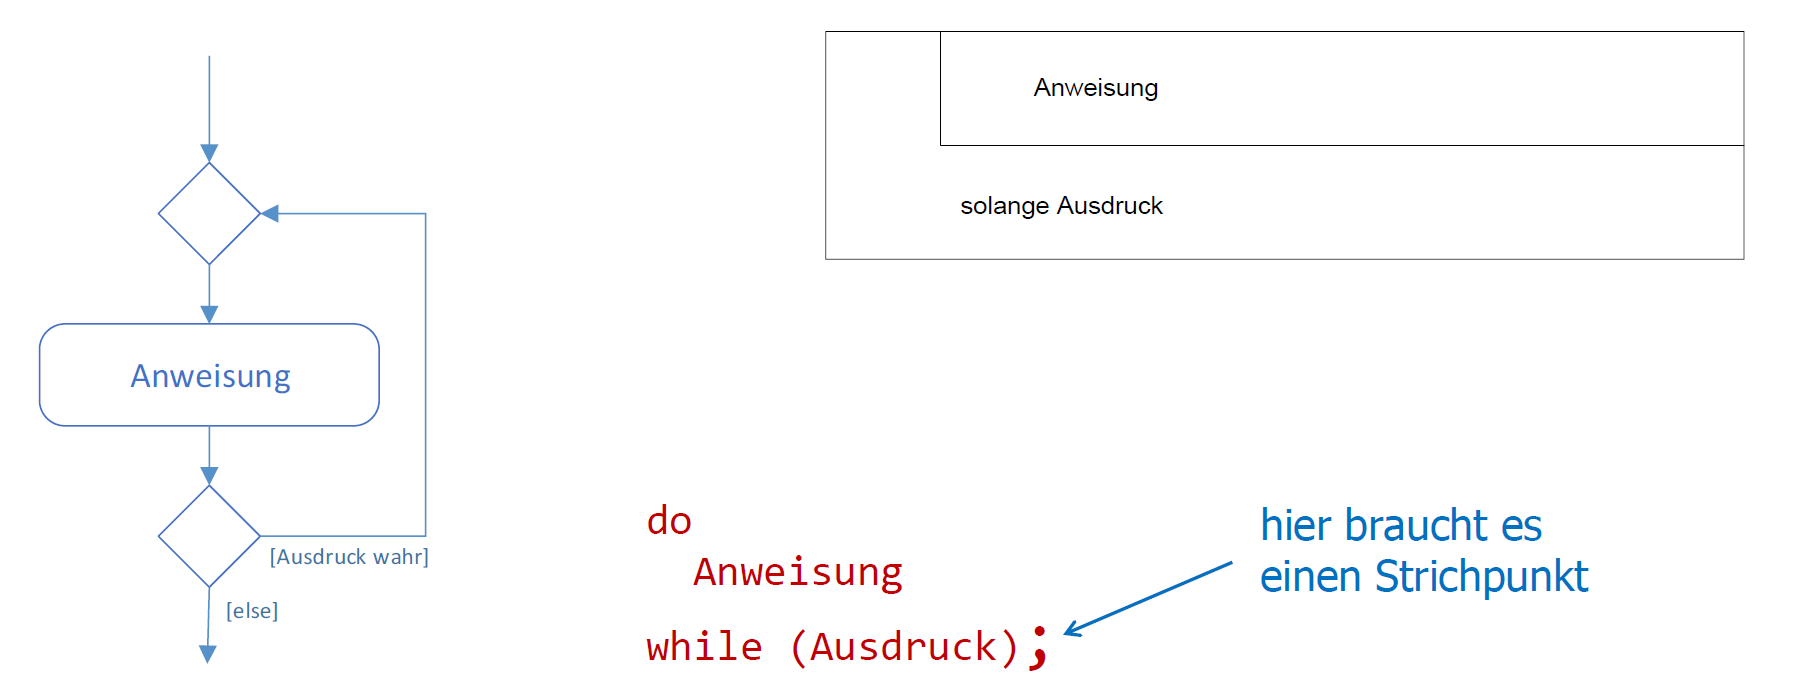
\includegraphics[width=0.95\linewidth]{Bilder/dowhile.png}
			\end{minipage}
			\hfill
			\begin{minipage}{.5\linewidth}
				Do-While-Schleife
			\end{minipage}

		\subsubsection{While-Schleife}
			\begin{minipage}{.45\linewidth}
				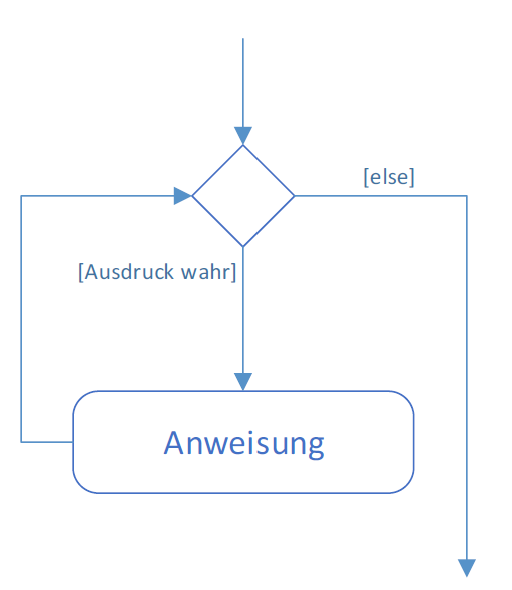
\includegraphics[width=0.5\linewidth]{Bilder/while1.png}
				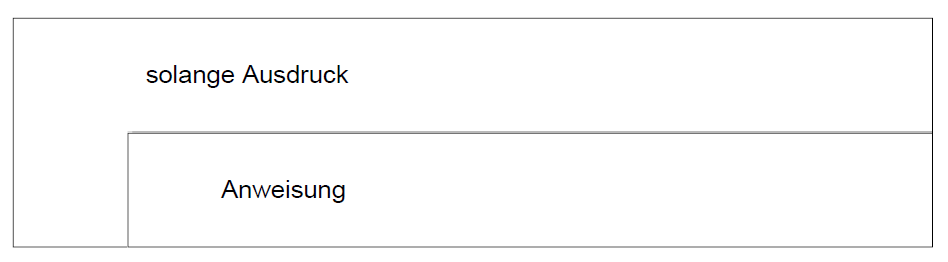
\includegraphics[width=0.5\linewidth]{Bilder/while2.png}
			\end{minipage}
			\hfill
			\begin{minipage}{.5\linewidth}
				While-Schleife
			\end{minipage}

		\subsubsection{Sprunganweisungen}
			\begin{itemize}
				\item \verb|break|: Schleifen abbrechen, zurückhaltend einsetzen!
				\item \verb|continue|: nächsten Schleifendurchgang starten, sehr zurückhaltend einsetzen!
				\item \verb|return|: aus Funktion zum Aufruf springen
				\item \verb|goto|: zu einer Marke springen, VERMEIDEN!
			\end{itemize}

	\subsection{Code-Snippets}
		\subsubsection{Array und Pointer}
			\begin{lstlisting}[language=C]
#include <stdio.h>

int main(){
	enum{array_size = 6};
	int test[array_size] = {1,2,3,4,5,6};
	for(int i =0; i<array_size; ++i)
		printf("Element %u: %i\n", i, test[i]);
	
	printf("Groesster: %d", *findAbsMax(test, array_size));
	return 0;
}
			\end{lstlisting}
			Main-Funktion zum Finden eines \textbf{betragsmässig} grössten Wertes innerhalb eines Arrays.

			\begin{lstlisting}[language=C]
int* findAbsMax(int* arr, size_t size){
	int* max_ptr = &arr[0];
	for(size_t i = 0; i < size; ++i){
		if((arr[i] >=0 && *max_ptr >=0 && arr[i] > *max_ptr)
		|| (arr[i] <=0 && *max_ptr <=0 && arr[i] < *max_ptr)
		|| (arr[i] >=0 && *max_ptr <=0 && arr[i] > *max_ptr * -1)
		|| (arr[i] <=0 && *max_ptr >=0 && arr[i] * -1 > *max_ptr))
			max_ptr = &arr[i];
	}
	return max_ptr;
}
			\end{lstlisting}